\documentclass[12pt]{article}
\usepackage{graphicx}
\usepackage{color}
\usepackage[letterpaper, margin=1.50in]{geometry}
\usepackage[utf8]{inputenc}
\usepackage[T1]{fontenc}
\usepackage[french]{babel}
\frenchbsetup{StandardLists=true}
\usepackage{enumitem}
\title{Travail pratique 1 - IFT-2245}
\author{Kevin Palmang Kombate et Mohamed Sarr}

\begin{document}

\maketitle
\newpage

\section{INTRODUCTION}\vspace{0,5cm}

 Ce travail pratique a visé à nous familiariser avec la programmation système dans un système d’exploitation de style POSIX.\\
 
Ce Shell est la représentation d’un Shell de base minimaliste de plusieurs fonctions implémentées tel que :
\begin{itemize}
\item  Exécution des commandes telles que echo, cat, man, tail.
\item Implémentation des statuts de transmission d’un processus avec \&\& et ||  
\item Implémentation des déclarations de « IF ».
\item Implémentation de la redirection de sortie et gestion de tâche arrière-plan avec \& et >
\end{itemize}
\vspace{0,3cm}

\section{NIVEAU DE L'ÉQUIPE}\vspace{0,5cm}

Notre équipe n’avait aucune expérience avec le langage de programmation C et a particulièrement trouvé ce travail pratique très demandant tant au niveau du temps que des concepts à maîtriser. 

La compréhension des notions principales de ce langage (attribution de mémoire, utilisation des pointeurs, appels système) était l’un des points qui nous a donné de fil à retordre lors de la réalisation.\\

Le concept de base de ce travail pratique étant également d’effectuer du parsing, nous avons fait de notre mieux malgré notre manque de connaissances dans le domaine.\vspace{0,3cm}


\section{DIFFICULTÉES RENCONTRÉES}\vspace{0,5cm}
L’un des tous premiers problèmes rencontrés avant l’implémentation de notre Shell étaient de comprendre le sujet et l’apprentissage du langage de programmation C.
Puis surviennent les problèmes liés à l’implémentation du Shell. Tout d’abord, comment attaquer le sujet? Quels stratèges opter l’implémentation et la compilation du code?

A cela s’ajoute les problèmes liés au bugs et le plus dure était de les tracer. Nous avons pu utiliser IDE CLion de JetBrains qui nous a permis de résoudre nos problèmes de syntaxes et de débogage.

Par la suite, nous avons été confrontés à comprendre pourquoi et quand faire une demande mémoire, pour la réutilisation d’une variable en dehors d’une fonction. De plus, nous avions de la difficulté à maîtriser le référencement des pointeurs, la création et l’utilisation de tableau de char au lieu du type String et d’autres concepts clés comme l’arithmétique des pointeurs.\\

 Ensuite, nous avons eu à comprendre les librairies du langage de programmation C afin de les utiliser dans les différents contextes auxquels nous devons faire face. Après des recherches, nous avons découvert strtok qui nous permet de séparer notre commande en token et d’y accéder par la suite. Toutefois, nous avions mal compris certaines caractéristiques du strtok, ce qui nous a fait du coup perdre un temps important.
 
Selon nous, la plus grande difficulté rencontrée durant l’élaboration du projet était de le structurer en plusieurs sous méthodes (fonctions). Vu la limitation des fonctions gérées par notre Shell il est certain qu’il soit minimaliste et pas mature.\\

Certaines problématiques que nous n’avions pas réussi à régler malgré notre bonne volonté sont :\\
\begin{enumerate}
\item \underline{Implémentation des statuts de transmission d’un processus avec \&\& et ||} \vspace{0,1cm}

Nous avons toutefois réussi à implémenter les processus avec les \&\& et || mais seulement lorsqu’il y a un seul des opérateurs dans l’input mais pas deux. (Voir Figure 1).\\

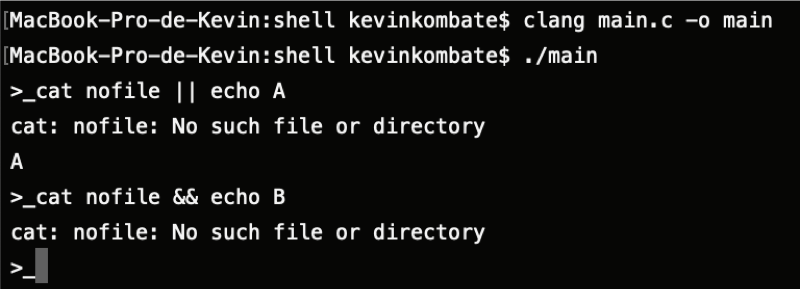
\includegraphics[scale=1]{fig1.png}
\title{Figure 1}\vspace{0,3cm}

Lorsqu’on décide de mettre les deux opérateurs dans le même input cela ne marche pas vu qu’il n’a pas été demandé de l’implémenter.\vspace{0,5cm}

\item \underline{Implémentation des déclarations de « IF »} \\

Les commandes de bases de la commande IF ont été implémenté avec succès et fonctionnent bien. Toutefois, certains tests ne se réalisent pas comme ils devraient. \\

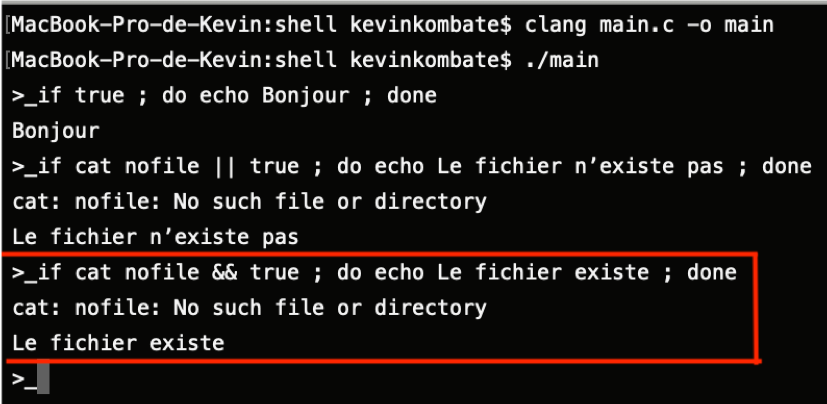
\includegraphics[scale=1]{fig2.png}
\title{Figure 2}
\newpage

Sur la Figure 2 la commande entourée en rouge devait exécuter que le « cat : nofile : No such file or directory » mais il exécute aussi la deuxième partie de la commande IF pour des raisons indépendantes de la nôtre (même si cela a bien été spécifié dans notre code).\\

Par contre, les commandes IF avec les opérateurs logiques || et \&\& ont été bien implémenté (Voir Figure 3).\\

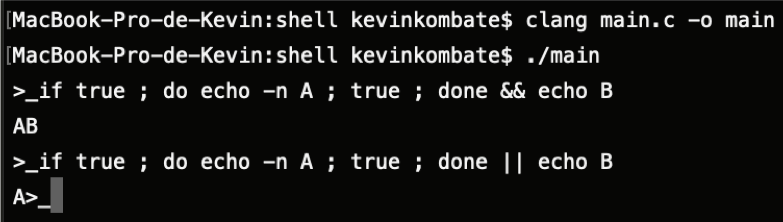
\includegraphics[scale=1]{fig3.png}
\title{Figure 3}\vspace{0,5cm}


\item \underline{Implémentation de la redirection de sortie et gestion de tache arrière-plan avec \& et >} \vspace{0,1cm}

En raison du temps et de l’effort fourni pour l’implémentation de la commande IF nous n’avons pas eu le temps et les ressources afin d’implémenter cette fonction dans notre Shell. Toutefois, nous avons laissé en commentaire dans notre code l’avancé que nous avons réalisé même si celui-là est minime.\\

{\color{red}NOTE: Pour l’exécution des IF, il faut mettre des espaces avant et après le « ; » (Mon découpage a été réalisé en fonction de cela).}\\

Du fait que la plupart de nos tests étaient fonctionnels, nous avons essayé de réorganiser au mieux notre code, de réécrire certaines demandes de mémoire et de libérer la mémoire non utilisée. 
\end{enumerate}\vspace{0,3cm}
\newpage

\section{CONNAISSANCES ACQUISES}\vspace{0,5cm}
Durant la réalisation de ce travail pratique, nous avons acquis de la connaissance sur trois points majeurs qui sont :
\begin{enumerate}
\item Le fait qu’on ai besoin d’un fork avant de exec si on désire qu’il ait un processus existant et que l’application ne meure pas.
\item Le fait qu’il faut envoyer un argument à wait si on veut récupérer le code d’exécution du child via le parent.
\item Le fait de demander de la mémoire grâce à malloc si on veut réutiliser une variable en dehors de son scope. 
\end{enumerate}\vspace{0,3cm}


\section{OUTILS UTILISÉS}\vspace{0,5cm}
Durant le développement du shell ous avons utilisés différents outils informatique: CLion(IDE en C et C++) de JetBrains; MacOs (en utilisant gcc pour la compilation); le siteWeb codeshare.io pour partage du code entre les membres de l'équipe; l'éditeur de texte Sublime Text et enfin latex pour la rédaction de ce magnifique rappport.\vspace{0,3cm}

\section{CONCLUSION}\vspace{0,5cm}
Pour conclure nous pouvons dire que ce projet nous a permis d'apprendre plus sur le langage C et sur l'utilisation des pointeurs et la manipulation des entrées sorties.Toutefois l'amélioration de notre shell demeurera une de nos priorité afin d'atteindre un Shell plus mature avec plus de fonctionnalités implémentées.

\end{document}
